\documentclass[a4paper,11pt]{article}

% Standart.
\usepackage[T1]{fontenc}
\usepackage[utf8]{inputenc}
\usepackage{lmodern}
\usepackage[french]{babel}
\usepackage{eurosym}

% Page format.
\usepackage{geometry}
\geometry{top=2cm, bottom=2cm, left=1cm, right=1cm}

% Figures.
\usepackage{graphicx}
\graphicspath{{resources/}}
\usepackage{float}
\usepackage{array}
\usepackage{tikz}

% Math and chemistry.
\usepackage{chemist}
\usepackage{siunitx}
\usepackage{numprint}
\usepackage{amsmath}
\usepackage{amssymb}
\usepackage{stmaryrd}
\usepackage{mathrsfs}

% Links. Should be loaded last.
\usepackage{hyperref}
\hypersetup{
  colorlinks=true,
  linkcolor=blue,
  filecolor=magenta,
  urlcolor=cyan,
  citecolor=blue}


% Dummy environment. Useful for some convoluted layouts.
\newenvironment*{dummyenv}{}{}

% Custom commands
\newcommand{\R}{\mathbb{R}}
\newcommand{\Z}{\mathbb{Z}}
\newcommand{\N}{\mathbb{N}}
\newcommand{\der}{\,\mathrm{d}}
\newcommand{\e}{\mathrm{e}}
\newcommand{\ti}{\cdot}

\title{Compression}
\author{Guillaume TOCHON}
\date{17 mars 2018}

\begin{document}

\maketitle
\tableofcontents

\section{Compression de données}

Site des slides : \url{www.lrde.epita.fr/~gtochon/CODO/}

Ces notes sont à travailler en parallèle avec les slides.

Compression + décompression

Sans compression de données, un film 720p d'une heure ferait presque 400Gio.

La naissance naïve de la compression de données remonte aux environs du code
morse.
Shannon est responsable des fondements mathématiques.

Autres acteurs:
  - Abraham Lempel
  - David Huffmann
  - Terry Welch

\

Le but de la compression est que lors de la décompression, ce soit le moins
visible possible par l'utilisateur.

\

\subsection{Sur la compressabilité}

\subsubsection{Entropie}

On va chercher a eliminer les redondances, et les gaspillages.
L'outil que l'on va utiliser est l'entropie.

Du point de vue de Shannon, plus un message est probable, moins il contient
d'informations.

\

Prenons un alphabet $\Sigma$ de $N$ symboles:
$$ \Sigma = \{s_1,s_2, ..., s_N\} $$

Avec leurs probabilités d'occurrence respectives:
$$ p_i = p(s_i) $$

Évidemment, on a
$$ \sum_{i = 1}^{N} p_i = 1$$

\

Soit $F$ un fichier composé de $N_F$ éléments de $ \Sigma $.

Statistiquement, $s_i$ est présent $p_i \times N_F$ fois.

On définit $q_i$ la quantité d'information totale d'un symbole:

$$ q(s_i) = -log_2(p_i) $$

On a donc $Q_{Tot}$ la quantité d'information propre totale de $s_i$ contenue
dans $F$, d'unité Sh/symbole, abrégée Sh/symb:

$$ Q_{Tot}(s_i) = -N_F \cdot p_i \cdot \log_2(p_i) \text{ Sh/symb}$$

On définit donc $Q_{Tot}(F)$ la quantité d'information contenue dans un fichier
$F$, d'unité Sh:

\begin{align*}
  Q_{Tot}(F) &= \sum_{i = 1}^{N_F}(Q_{Tot}(s_i) \\
             &= \sum_{i = 1}^{N_F} -N_F \ti p_i \ti \log_2(p_i) \\
             &= -N_F \sum_{i = 1}^{N_F}p_i \ti \log_2(p_i) \text{ Sh}
\end{align*}

Or ce $-N_F$ devant la somme pose problème:  \textbf{la quantité d'information
  dépend de la taille du fichier}.

Cela implique qu'un gros fichier ``probable'' contient moins d'information qu'un
petit fichier improbable.

\

On définit donc l'entropie $H$ ainsi:

$$ H = \frac{Q_{Tot}(F)}{N_F} = - \sum_{i = 1}^{N_F}p_i \ti \log_2(p_i)$$

\

On notera en outre que:

$$ H \equiv Sh $$

\

On remarquera que l'entropie $H$ est \textbf{indépendante} de la taille du
fichier.

$H$ ne dépend donc que de l'alphabet considéré $\Sigma$ et de la distribution
des symboles qui compose le fichier $F$.

\subsubsection{Probabilités}

Soit $X$ une variable aléatoire telle que:

$$ X = \{x_1, x_2 ..., x_n\}$$

Et

$$ p_i = P(X = x_i) $$

On a donc l'espérance de $X$:

$$ E(X) = \sum_{i = 1}^nx_i \ti p_i = \sum_{i = 1}^nx_i \ti P(X = x_i) $$

Et on a donc:

$$ E(\varphi(X)) = \sum_{i = 1}^n \varphi(x_i) P(X = x_i) $$

\

On a donc, pour l'entropie:

\begin{align*}
  H &= - \sum_{i = 1}^{N_F}p_i \ti \log_2(p_i) \\
    &= \sum_{i = 1}^{N_F} \underbrace{(- \log_2(p_i))}_{q_i} \ti p_i \\
    &= \sum_{i = 1}^{N_F} q_i \ti p_i \\
    &= E(q(s_i))
\end{align*}

\subsubsection{Application à l'informatique}

On considère donc:

\begin{align*}
  N_\Sigma &= \{0, 1\} \\
  p(0) &= p_0 = p \\
  p(1) &= p_1 = 1 - p
\end{align*}

On a alors:

\begin{align*}
  H &= -p \ti \log_2(p) - (1 - p) \log_2(1 - p) \\
    &= H(p)
\end{align*}

Par convention, on pose:

$$ H = - \sum_{i = 1}^{N_F}p_i \ti \log_2(p_i) $$

$$ p_i \ti \log_2(p_i) = 0 \text{\quad si \quad} p_i = 0 $$

\subsubsection{Cas de l'entropie nulle (À corriger avec le prof)}

$H(0) = H(1) = 0$

On a des fichiers complètement désordonnés:

$$ p = 0 \implies F = \{1111...1\} $$

$$ p = 1 \implies F = \{0000...0\} $$

Donc l'entropie est nulle.


\

Quand $p = \frac{1}{2}$, les symboles sont équiprobables, le fichier est
complètement désordonné, donc complètement aléatoire. Dans ce cas, l'entropie
est donc \textbf{maximale}.

\

Voir la figure \ref{entropy_prob}.

\begin{figure}[!h]
  \centering
  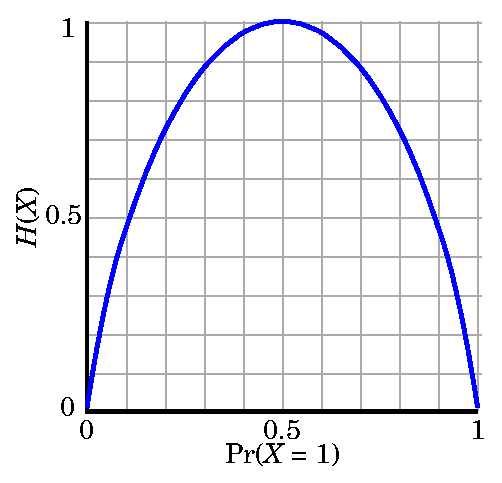
\includegraphics[width = 0.5 \textwidth]{Binary_entropy_plot.eps}
  \caption{Entropie en fonction de $P(X = 1)$}
  \label{entropy_prob}
\end{figure}

\

Attention! L'entropie ne voit pas les méta-symboles! Par exemple, ce fichier
est considéré comme parfaitement alétaoire:

$$ F = \{01010101\} $$

\subsubsection{Calcul de l'entropie}

Soit l'alphabet

$$ \Sigma = \{s_1, s_2, ..., s_N\} $$

De longeur:

$$ \forall n \in \N, \quad N_{\Sigma}= 2^n $$

Avec:

$$ \forall s_i \in \llbracket 1, N_{\Sigma} \rrbracket, \quad p(s_i) = p_i = \frac{1}{N_{\Sigma}} $$

On a donc:

\begin{align*}
  H &= - \sum_{i = 1}^{N_{\Sigma}}p_i \ti \log_2(p_i) \\
    &= - \sum_{i = 1}^{2^n} \frac{1}{2^n} \ti \underbrace{\log_2\left(\frac{1}{2^n} \right)}_{- n} \\
    &= \frac{1}{2^n} (-n) \underbrace{\sum_{i = 1}^{2^n} 1}_{2^n} \\
    &= n
\end{align*}

\subsubsection{Exercice}

VÉRIFIER AVEC LE PROF!

\

De combien de bits a-t-on besoin pour encoder le fichier suivant?

$$ F = \{ACABBDDBAAABCAAA\} $$

Dans ce cas, on utilisera l'alphabet suivant:

$$ \Sigma = \{A, B, C, D \} $$

Comptons le nombre d'occurrences de chacune des lettres de $ \Sigma $:

\[\left.
  \begin{array}{lr}
    A: & 8 \\
    B: & 4 \\
    C: & 2 \\
    D: & 2
  \end{array}
\right\} \quad \text{Longeur: 16}
\]


\begin{enumerate}

\item Non compressé?

  C'est tout simplement, en notant $\Sigma$ l'alphabet utilisé pour encoder le
  fichier,

  \begin{align*}
    \text{Résultat} &= \text{Longeur} \times \text{Nombre de bits nécessaire
                      pour encoder } \Sigma \\
                    &= 16 \ti \log_2(n_{\Sigma}) \\
                    &= 16 \ti \log_2(4) \\
                    &= 32 \text{ bits}
  \end{align*}

\item Compressé?

  Calculons l'entropie du fichier:
  \begin{align*}
    H &= p_A \ti \log_2(p_A) + p_B \ti \log_2(p_B) + p_C \ti \log_2(p_C) + p_D \ti \log_2(p_D) \\
      &= \frac{1}{2} \ti \log_2\left(\frac{1}{2}\right) + \frac{1}{4} \ti \log_2\left(\frac{1}{4}\right) +
        \frac{1}{8} \ti \log_2\left(\frac{1}{8}\right) + \frac{1}{8} \ti \log_2\left(\frac{1}{8}\right) \\
      &= \frac{7}{4}
  \end{align*}

  Donc la longeur totale minimale du message est:

  \begin{align*}
    \text{Résultat} &= \text{Longeur} \times H \\
                    &= 16 \ti \frac{7}{4} \\
                    &= 28 \text{ bits}
  \end{align*}

\end{enumerate}

\section{Algorithmes de compression conservatifs}

\subsection{Run-length encoding}

Pas génial pour le texte.

Mieux pour les images de synthèse. C'est utilisé dans bitmap.

Le principe c'est de coder combien de fois on voit chaque caractère.

Pour les nombres, caractère spécial.

\subsubsection{Cas du fax}

C'est utilisé pour le fax et ça marchait bien car il y a beaucoup de blanc.

On peut même compresser la différence entre deux lignes consécutives pour gagner
de la place.

C'est une technique très largement utilisée, par exemple dans JPEG et MPEG.

\subsection{Algorithme d'Huffman}

Un des algorithmes les plus célèbres.

Code entropique: il est basé sur la distribution statistique des symboles.

\

Deux étapes:

\begin{enumerate}
\item Construction d'un arbre binaire donc les feuilles sont les symboles.
\item Encodage du message avec cet arbre.
\end{enumerate}

\

Première étape:

\begin{enumerate}
\item Trier la table
\item Fusionner les deux symboles
\end{enumerate}

Seconde étape:

\begin{enumerate}
\item Parcourir l'arbre de la racine vers les veuiulles (les symboles)
\item Toujours assigner 1 au fils gauche et 1 au fils droit (ou l'inverse)
\item Lire l'encodage sur la branche entière.
\end{enumerate}

\

C'est un encodage à préfixe donc on peut le décoder à la volée. Il est optimal à
la longeur d'encodage moyenne parmi les encodages à préfixe. Il nous donne
exactement l'entropie tant que que les symboles sont une puissance de 2.

\

Problème: c'est de l'encodage symbole par symbole.

\

De nos jours, on ne s'en sert pas tel quel, mais en conjonction avec des
algorithmes plus complexes.

\subsection{L'algorithme bzip2}

Libre et open-source, créé entre 1996 et 2000. Grosse usine à gaz.

L'idée:

\begin{enumerate}
\item Appliquer la transformée de Burrows-Wheeler. Cela change l'ordre des
  caractères pour former des suites de caractères identiques, tout en restant
  réversible à la décompression.

  \

  Encodage:
  \begin{itemize}
  \item Contruire une matrice contenant toutes les rotations de la string à
    transformer.
  \item Trier les colonnes selon l'ordre alphabétique.
  \item Stocker la rotation de la matrice et ces colonnes.
  \end{itemize}

  \

  Décodage:

  \begin{itemize}
  \item Concaténer les chaîne avec la dernière colonne de la table.
  \item À céompléter
  \end{itemize}

\item La transformée ``Move to front''

\item Algorithme d'Huffman.

\end{enumerate}

\

Problème: lent à la compression, mais très économe en place. Très efficace pour
langage naturel, pas trop pour du code.

\subsection{Algorithme LZW}

On a intérêt à le refaire sur papier pour bien le comprendre.

C'est le premier algorithme, avec LZ78, qui fasse de l'aprentissage de
dictionnaire non-supervisé.

Voir le processus sur les diapos.

C'est utilisé dans GIF.

\section{Conversion analogique-digitale}

\subsection{Un petit exemple}

On prend un fichier audio que l'on ouvre avec Audacity pour voir que le fichier
ressemble toujours à un entité continue de loin mais discrète de près.

C'est une pression qui dépend de l'espace et du temps.

On considère notre tension avec la varaible $f_a : \R \rightarrow \R$.

Que l'on va discrétiser ainsi: $f_d: \Z \rightarrow \R$.

\subsection{Le problème de l'échantillonage}

Voir slides.

On prend des points $(t_n)_{n \in \Z}$ pour faire la séquence

$$(f_d(n) = f_a(t_n))_{n \in \Z}$$

Pour faire simple, on prend des points à un intervalle régulier. On a donc

$$ t_n = nT_e $$

$T_e$ : Période d'échantillonage

$f_e = \frac{1}{T_e}$ : Fréquence d'échantillonage

Il faut la choisir avec soin pour avoir un bon compris taille/qualité.

\subsection{À quelle vitesse un signal varie-t-il?}

On va faire une représentation fréquentielle puisque la représentation
temporelle ne convient pas. Cette représentation est une \textbf{transformée de
 Fourier}.

Elle prend beaucoup moins de place et représente la même information.

Comment y arrive-t-on?

\subsubsection{La transformée en séries de Fourier. [Compléter]}

Elle s'écrit:

$$ c_n = \frac{1}{T} \int_0^T x(t) \e ^{-2 i \pi \frac{n}{T} t} \, \text{d} t $$

Elle s'applique pour des raisons physiques.

\

Prenons un exemple simple:

Soit une fonction carrée de période T:

\[ f(t) =
\begin{cases}
  1 &\text{si t} \in [0, \frac{T}{2}] \\
  0 &\text{si t} \in [\frac{T}{2}}, T]
\end{cases} \]

\

On a

$$ \tilde{f}  = \frac{1}{2} + \sum^N_{n = 1} $$

\subsubsection{Le produit scalaire}

Voir le poly.

Le produit scalaire $<x, y>$ entre deux éléments $(x, y) \in E \times E$

Dans $E = \R ^2$:

$$<x, y> = ||x|| ||y|| \cos{\theta}$$

Dans $E = \R ^ n$:

\[ x = \left( \begin{matrix} x_1 \\ \vdots \\ x_n \end{matrix} \right) =
\sum^n_{i = 1} x_i \cdot u_i = \sum^n_{i = 1} \]

Dans $E = \math{L}$:

\subsubsection{Illustration géométrique de la décomposition en série de Fourier}

\subsubsection{La décomposition en série de Fourier}

\begin{align*}
  f(t) &= \sum^{+ \infty}_{- \infty} c_n \e ^{i 2 \pi \frac{n}{T} t}\\
       &= a_0 + \sum^{+ \infty}_{n = 1} a_n \cos(2 \pi \frac{n}{T} t) + b_n \cos(2 \pi \frac{n}{T} t)
\end{align*}

\subsubsection{La transformée de Fourier}

\begin{align*}
  c_n = \frac{1}{T} \int_0^T f(t) \e ^{-2}
\end{align*}

On a

$$ \mathcal{F}(f \times g) = \mathcal{F}(f) * \mathcal{F}(g) $$

\subsubsection{Propriétés pratiques du Dirac}

$$f(t) \times \delta(t - t_0) = f(t_0) \times \delta (t - t_0) $$

C'est l'élément neutre du produit de convolution.

$$ f(t) = \delta (t - t_0) = f(t - t_0) $$

Voir le reste sur les diapos.

\subsubsection{Après le peigne de Dirac}

\begin{align*}
  \tilde{f_d} = f_a \times W_{T_e} (t)
\end{align*}

\begin{align*}
  \mathcal{F}(\tilde{f_d}) &= \mathcal{F}(f_a \times W_{T_e}) \\
                           &= \underbrace{\mathcal{F}(f_a)}_{\tilde{f}_a(u)} \times \mathcal{F}(W_{T_e}) \\
                           &= 
\end{align*}

\subsubsection{Effet stroboscopique}



\end{document}
